%% ------------------------------------------------------------------------- %%n
\chapter{Experimentos e Resultados Preliminares}
\label{cap:Experimentos_Resultados}


Nesse capítulo serão apresentados alguns experimentos preliminares que foram feitos com dados sintéticos e com dados reais de plâncton. 

\section{Framework de Aprendizado Ativo Utilizado}
\label{sec:framework_al}

O framework utilizado nesses experimentos foram baseados no trabalho de \citep{saito2014active}. A figura~\ref{fig:priscila_algoritmo} e os seguintes passos explicam as etapas:

\begin{figure}
  \centering
  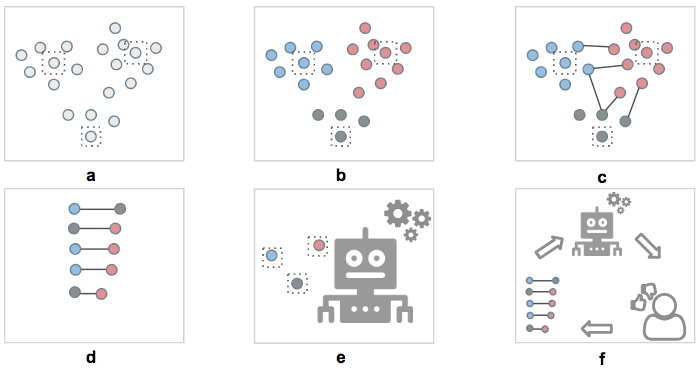
\includegraphics[width=1.0\textwidth]{figures/priscila_algoritmo.png}
  \caption{Framework Utilizado nos Experimentos}
  \label{fig:priscila_algoritmo}
\end{figure}




\begin{enumerate}
  \item No primeiro quadro (a), temos um conjunto de dados em um espaço de características. Inicialmente esses dados não estão rotulados, então não sabemos quais são suas classes. Temos a informação sobre quantas classes podem existir para esses dados;
  
  \item Em (b), apenas para ilustração, temos as verdadeiras classes dos dados;
  
  \item Em (c), aplicamos um algoritmo não-supervisionado de clusterização. No nosso caso utilizamos o algoritmo K-means e consideramos o número de classes $k$ como sendo o dobro do número de classes possíveis. No exemplo, supomos que são 2 classes, logo consideramos $k=4$; 
  
  \item Em (d), aplicamos o algoritmo de vizinhos mais próximos K-NN em todos os dados para gerarmos um grafo. O número de vizinhos foi escolhido de forma prática. 
  

  \item Em (e), como temos os clusters, reduzimos o dataset original para os dados que possuem vizinhos pertencentes a clusters distintos. Note que as amostras que possuiam como vizinhos dados do mesmo cluster estão um pouco apagados. Na realidade, elas não serão consideradas no dataset reduzido. A ideia é que tenhamos apenas os dados que estejam na borda dos clusters pois eles são mais informativos. As amostras que possuem um pontilhado em volta representam os centróids de cada cluster e eles também compõem o dataset reduzido;
  
  \item Em (f), ordenamos as amostras do dataset reduzido, de maneira decrescente, segundo a distância euclidiana das arestas. Iniciamos por elas pois temos como premissa que uma maior distância pode representar amostras mais relevantes;
  
  \item Nos quadros (g) e (h), %como sabemos os rótulos verdadeiros dos dados, geramos um classificador através dos centroides dos clusters. Esses dados compõe um novo dataset que será utilizado como base de treinamento. 
  \NINA{os centróides dos clusters são rotulados, compondo o conjunto inicial T. Um classificador é treinado a partir de T. Na prática, essa rotulação pode ser obtida por meio de consulta ao oráculo, mas em uma simulação sabemos a classe de cada amostra e esse conhecimento é usado para simular um oráculo.}
  A partir desse ponto entramos no ciclo do Aprendizado Ativo. A cada início de ciclo, selecionamos $n$ amostras do dataset reduzido e o classificador gera as predições para essas amostras. A consulta ao oráculo é simulada comparando-se a classificação atribuída pelo classificador com os rótulos verdadeiros. Caso a classe esteja incorreta, corrigimos a classe. Incorporamos amostras selecionadas para a base de treinamento T. Esse ciclo continua até que os dados disponíveis no dataset reduzido acabem. 
\end{enumerate}

\NINA{Note que a redução do conjunto de dados não rotulados realizada no início do processo visa apenas reduzir o custo computacional.}

No caso da seleção aleatória, seguimos a mesma lógica até o passo 3 inclusive. A partir disso, geramos um classificador também usando os centróides e iniciamos o ciclo de aprendizado ativo. A cada ciclo, selecionamos $n$ dados não rotulados de forma aleatória.

\section{Experimentos com Dados Sintéticos}
\label{sec:experimentos_sinteticos}

Para os experimentos com dados sintéticos, geramos um dataset com 1000 amostras que representam um espaço de características 2D. A figura~\ref{fig:exemplo_sintetico_1} mostra do lado esquerdo os dados gerados sem informação de classe, enquanto o lado direito mostra os rótulos de classe. 


\begin{figure}
  \centering
  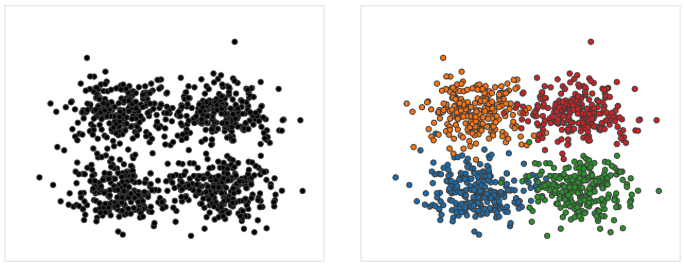
\includegraphics[width=0.9\textwidth]{figures/toy_example_1.png}
  \caption{Exemplo sintético}
  \label{fig:exemplo_sintetico_1}
\end{figure}

Aplicamos o framework anterior neste dataset. Como temos como premissa que são quatro classes possíveis, utilizamos no K-means oito clusters. A partir disso aplicamos o algoritmo de K-NN e obtemos a relações de interesse, conforme a figura ~\ref{fig:exemplo_sintetico_2}. 

\begin{figure}
  \centering
  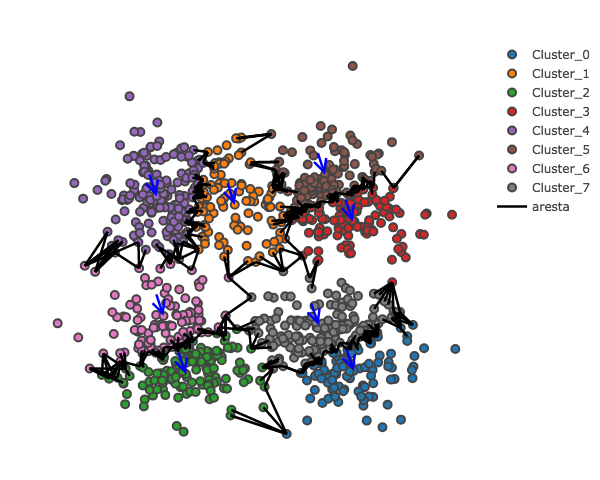
\includegraphics[width=0.8\textwidth]{figures/toy_example_2.png}
  \caption{Exemplo Sintético}
  \label{fig:exemplo_sintetico_2}
\end{figure}

É interessante notar que algumas amostras podem não ser tão relevantes pois pertencem ao mesmo grupo. Por exemplo, os clusters laranja (1) e roxo (4), na imagem ~\ref{fig:exemplo_sintetico_2}, são de fato uma única classe. Apesar disso, como o classificador será treinado inicialmente com o centroide de cada classe, é provável que a predição convirja rapidamente. De qualquer forma, os dados mais relevantes estão entre as amostras que não são da mesma classe. 


\begin{figure}
  \centering
  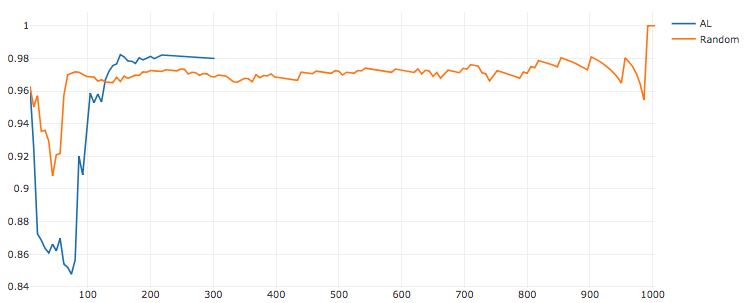
\includegraphics[width=0.9\textwidth]{figures/grafico_exemplo_sintetico.png}
  \caption{Gráfico com Resultados dos Dados Sintéticos}
  \label{fig:grafico_exemplo_sintetico}
\end{figure}

Fizemos os testes com a abordagem de seleção descrita acima e também com a seleção aleatória.  Escolhemos dez vizinhos próximos para encontrar as arestas e isso nos gerou um total de 300 dados, o que representa um redução de 70\% do dataset original. O gráfico da figura~\ref{fig:grafico_exemplo_sintetico} mostra a performance de ambas estratégias de seleção. É interessante notar que inicialmente o framework de Aprendizado Ativo não possui uma boa acurácia mas, após algumas amostras, entra numa sequência crescente, chegando em 98\% com 302 amostras. Em contraste, quando selecionamos os dados de forma randômica chegamos em 96.88\%. Além disso, com os dados aleatórios, atingimos um valor de 98\% apenas a partir de 900 amostras. Apesar de ambos os resultados terem uma boa taxa de acerto (provavelmente por ser um exemplo simples), o framework de Aprendizado Ativo mostrou a mesma taxa de acerto que a seleção aleatória com apenas 1/3 de amostras. 


\section{Experimentos com Dados de Plâncton}
\label{sec:experimentos_plancton}

Para os experimentos com imagens de plâncton, utilizamos parte da base de dados da FURG, consistindo de 1415 amostras de 6 classes. A figura~\ref{fig:Plancton_Exemplos} mostra alguns exemplos de imagens.


\begin{figure}
  \centering
  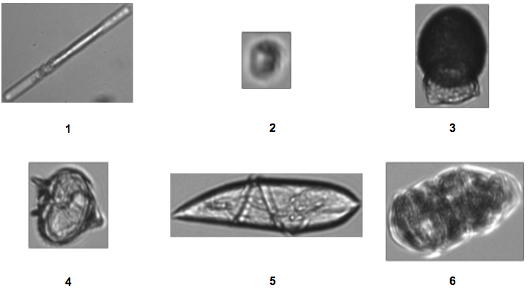
\includegraphics[width=0.6\textwidth]{figures/Plancton_Exemplos.png}
  \caption{Exemplos de imagens de plâncton utilizadas. As classes são 1:Bacillariophycidae-1, 2:Prorocentrales, 3:Spirotrichea, 4:Peridiniales, 5:Gymnodiniales, 6:Cochlodinium}
  \label{fig:Plancton_Exemplos}
\end{figure}

Essas 1415 imagens foram processadas por uma rede convolucional NASnet pré-treinada sobre o ImageNet, conhecido dataset público para classificação e detecção de objetos em imagens naturais, para a extração de características. Especificamente, os $n=4032$ valores da última camada antes da camada de classificação foram tomadas como as características de cada imagem.

Para o cálculos dos clusters, o algoritmo K-means foi utilizado com $k=12$, seguindo a mesma lógica de termos o dobro de clusters em relação ao número de classes. Para a redução do conjunto de dados iniciais, no cálculos dos vizinhos mais próximos foi utilizado o valor de 8. \TODO{Após esse processo, o conjunto inicial foi reduzido para 900 amostras.}


\begin{figure}
  \centering
  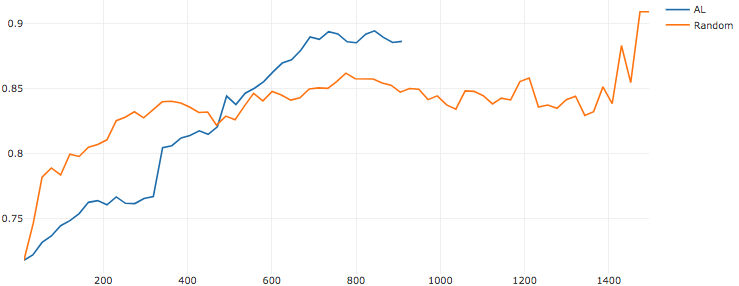
\includegraphics[width=0.9\textwidth]{figures/grafico_exemplo_plancton.png}
  \caption{Gráfico com resultados sobre as imagens de plâncton}
  \label{fig:grafico_exemplo_plancton}
\end{figure}

Assim como ocorreu no caso do exemplo sintético, os resultados mostram que, nas primeiras iterações, o aprendizado ativo é inferior ao método aleatório mas, a partir da iteração 22, com 471 dados, os dois métodos apresentam a mesma acurácia de 82\%. Desta iteração em diante o método de aprendizado ativo apenas melhora sua performance, enquanto o método aleatório permanece em uma tendência constante. No final, com cerca de 900 amostras, o método de aprendizado ativo atinge uma acurácia de 88.62\%. O método aleatório só atinge essa mesma acurácia com cerca de 1400 amostras. Isto é, o aprendizado ativo atinge a mesma acurácia com 2/3 do esforço.


\NINA{É importante notar que o algoritmo de seleção empregado tem suas particularidades e pode não ser adequado para o problema em questão. Um aspecto particularmente crítico é a redução realizada inicialmente. Caso a fronteira de decisão correta esteja realmente próxima ao conjunto reduzido de amostras então uma boa acurácia poderá ser obtida. Porém, em caso contrário, o conjunto reduzido não conterá todas as amostras informativas.}

\NINA{Há uma relação direta entre o número de clusters e o número de amostras no conjunto reduzido. Por um lado, é desejável considerar um número maior de clusters a fim de contemplar todos os pontos informativos, mas por outro lado isso pode resultar em um conjunto não tão reduzido de amostras a serem usadas no ciclo de aprendizado ativo, impactando no desempenho computacional. Desta forma, é bastante compreensível por que há várias variantes de algoritmos de aprendizado ativo.} 